\documentclass[french]{article}
\usepackage[T1]{fontenc}
\usepackage{fullpage}
\usepackage{babel}
\usepackage{hyperref}
\usepackage{graphicx}
\usepackage[justification=centering]{caption}
\usepackage{amsmath}
\usepackage{amssymb}
\usepackage{parskip}

\setlength{\parindent}{0pt}

\hypersetup{
  colorlinks=true,
  linkcolor=black,
  urlcolor=blue
}

\graphicspath{ {./img/} }
\title{%
    \huge Mathfinder  \\
    \bigskip
    \large E5 - Cas pratique \\ 
    Développeur en Intelligence Artificielle,
    titre professionnel enregistré au RNCP - École IA Microsoft by Simplon
    \vfill
    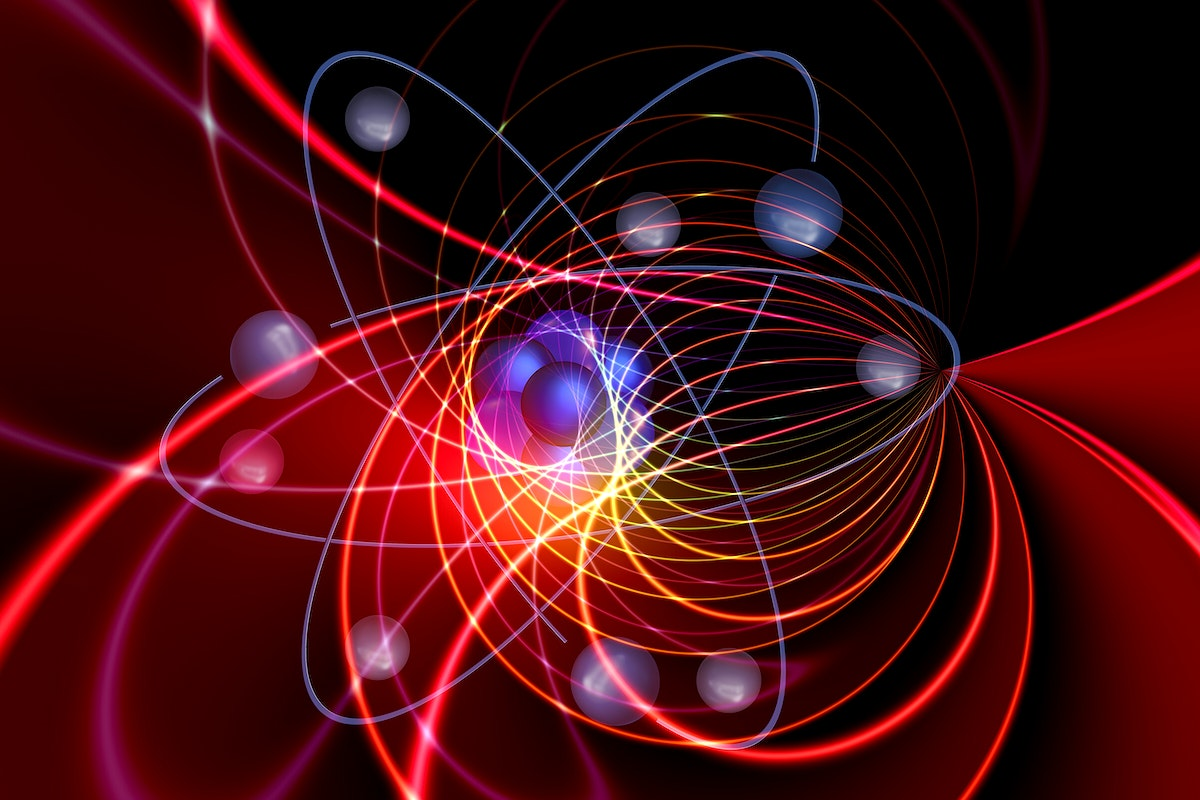
\includegraphics[width=14cm]{physics.jpg} % also works with logo.pdf
    \vfill}
\date{26 février 2024}
\author{par Vincent Papelard}

\begin{document}
    \renewcommand{\contentsname}{Table des Matières}
    \maketitle
    \pagenumbering{arabic}
    \pagenumbering{gobble}
    \newpage
    \tableofcontents
    \newpage
    \pagenumbering{arabic}

    \section{Contexte}
    Nous sommes les développeurs de Mathfinder, une application web à destination des physiciens. Mathfinder utilise une intelligence artificielle afin de calculer la fonction mathématique qui explique le mieux les données issues de leurs observations. L'application est destinée à être déployée directement sur les serveurs des établissements de recherche, qui réalisent les calculs.

    \begin{figure}[h]
        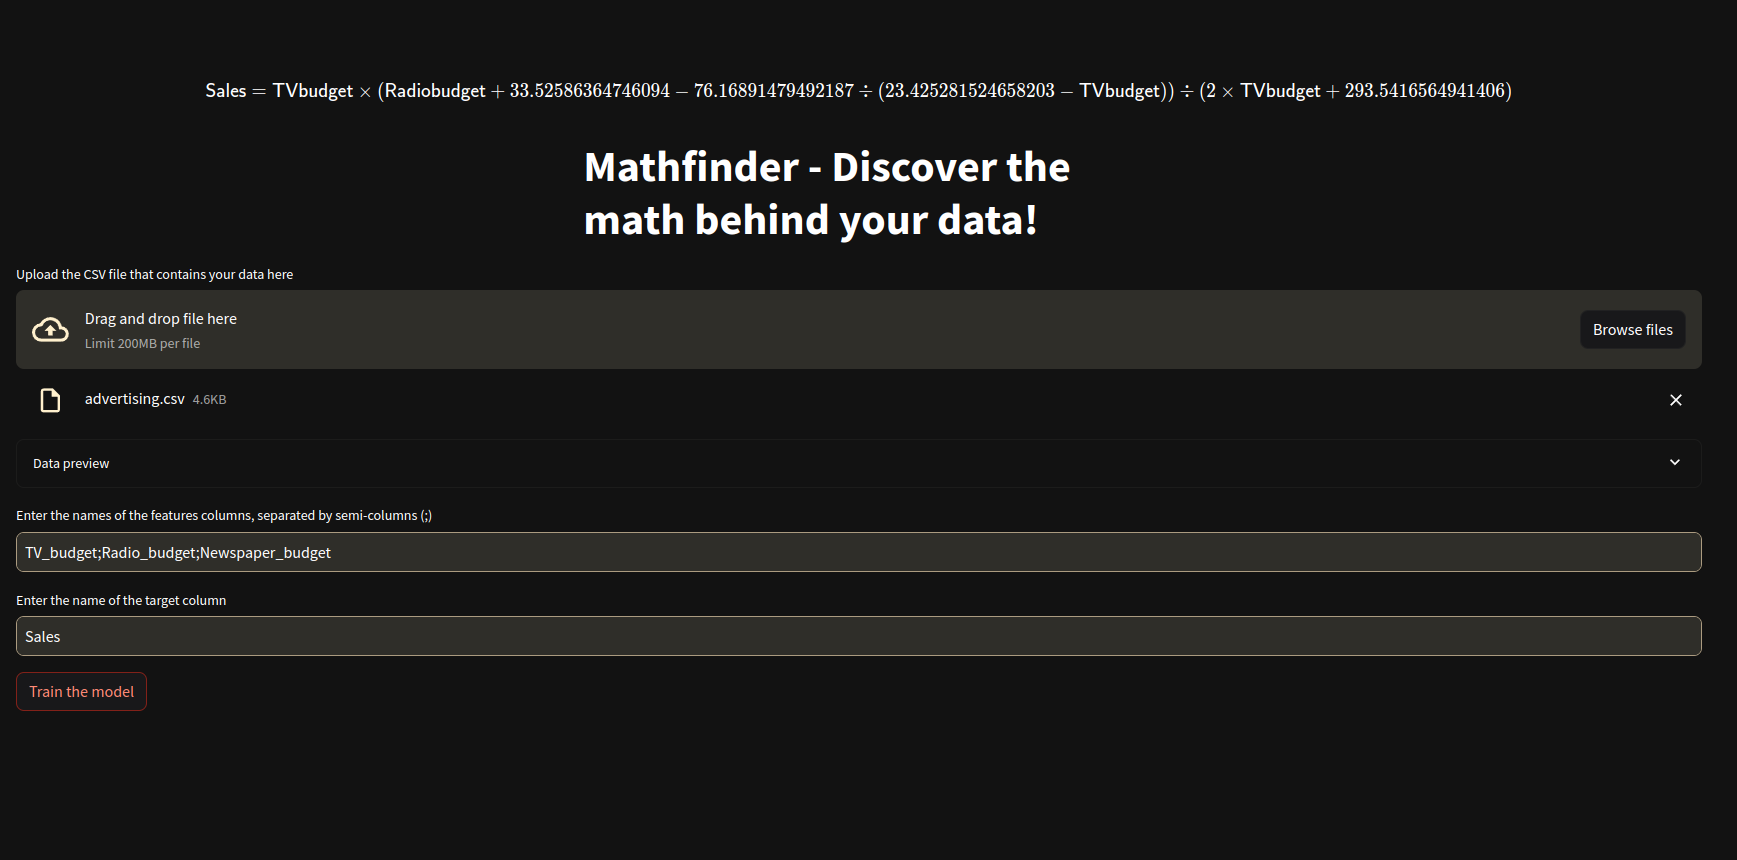
\includegraphics[width=12cm]{appli}
        \centering
        \caption{Mathfinder cherche une formule mathématique qui décrit les relations entre les données que l'on uploade. L'utilisateur peut entraîner un modèle sur ses propres données. Ce modèle est ensuite enregistré dans l'application et peut être réutilisé pour faire des prédictions}
        \centering
    \end{figure}

    Le directeur d'une grande université nous contacte. Les chercheurs de cette université ont récemment déployé Mathfinder sur leurs serveurs, mais plusieurs d'entre eux ont rencontré un problème étrange : la précision de leurs modèles d'IA se dégrade avec le temps ! Perplexe, le directeur se tourne vers nous pour que nous réglions ce problème. Par ailleurs, plusieurs bugs ont été rencontrés par les utilisateurs. Il exige que nous corrigions ces bugs et nous envoie un descriptif de tous les problèmes rencontrés :
    \begin{itemize}
        \item L'application crash quand on essaie de lui faire prédire les valeurs de deux colonnes ou plus
        \item L'application crash si on ne sépare pas le nom de chaque colonne avec des points-virgules \textbf{sans espace avant ou après}
        \item L'application crash s'il manque des valeurs dans certaines colonnes dans le fichier CSV fourni.
    \end{itemize}
    
    Ce dossier comporte deux volets :
    \begin{itemize}
        \item La mise en place de mécanismes de surveillance des modèles et d'alerte
        \item Le débugging des problèmes rencontrés, de la reproduction du bug à sa résolution.
    \end{itemize}
    Le code associé à ce projet est disponible \href{https://github.com/vinpap/mathfinder}{sur GitHub}. De plus, des captures d'écran sont disponibles en \hyperref[sec:annexes]{annexes} de ce dossier pour illustrer les différents mécanismes présentés.

    \section{Systèmes de surveillance des modèles}
    Commençons par traiter le premier problème signalé : la dégradation des performances des modèles d'intelligence artificielle au fil du temps. Ce phénomène apparaît lorsque les relations entre les variables de nos données ou leur distribution statistique ont changé depuis que notre modèle a été entraîné. On parle de \textbf{data drift} ou \textbf{concept drift}, selon les cas. 
    Quelle que soit la cause de ce "drift", il est important de pouvoir le détecter afin de réentraîner le modèle, si nécessaire. Nous allons maintenant voir comment mettre en place un système de suivi qui implémente les mécanismes suivants :
    \begin{itemize}
        \item \textbf{test automatique} des modèles d'IA entraînés pour voir si leurs performances se sont dégradées
        \item \textbf{alerte automatique par e-mail} en cas de dégradation des performances
        \item mise à disposition d'un tableau de bord qui permet aux gestionnaires de Mathfinder de \textbf{visualiser en détail} les performances de tous les modèles enregistrés.
    \end{itemize}
    \subsection{Outils utilisés}
    Les outils et plateformes suivants ont été utilisés afin de réaliser le monitorage de Mathfinder :
    \begin{itemize}
        \item \textbf{MySQL} est utilisé pour stocker les informations entrées par les utilisateurs lorsqu'ils entraînent un modèle (adresse e-mail et fréquence de test du modèle souhaitée). Nous choisissons d'utiliser MySQL car il est très simple à installer et mettre en place, ce qui simplifie le travail de notre client.
        \item Un \textbf{serveur SMTP} est nécessaire afin de pouvoir envoyer des alertes par e-mail. Dans le cadre de ce dossier nous avons utilisé le \textbf{serveur SMTP fourni par GMail}, mais notre client est libre d'utiliser le serveur qu'il souhaite lorsqu'il installe Mathfinder. La librairie Python \textbf{smtplib} nous permet quant à elle de communiquer avec le serveur SMTP.
        \item \href{https://mlflow.org/}{MLflow}, une plateforme qui permet de gérer le cycle de développement de modèles de machine learning. Nous l'utilisons afin de permettre à notre client de pouvoir visualiser simplement les performances des modèles entraînés par les utilisateurs de son organisation sur une interface graphique.
        
    \end{itemize}
    \subsection{Métrique de mesure des performances}
    \label{sec:metrics}
    Afin de pouvoir évaluer les performances des modèles d'intelligence artificielle des utilisateurs de Mathfinder, nous devons définir une métrique qui nous permet de les mesurer. Nous déciderons ici d'utiliser \textbf{l'erreur absolue moyenne} (souvent abrégée "MAE" pour \textit{Mean Absolute Error}). L'erreur absolue moyenne se définit comme la moyenne des erreurs obtenues par un modèle :

    \begin{figure}[h!]
        \begin{equation}MAE = \frac{\sum \lvert A-P \rvert}{N}  \end{equation}
        \centering
        \caption{Définition de la MAE. Ici $N$ représente le nombre total de prédictions réalisées, $A$ est la valeur réelle, et $P$ la valeur prédite par le modèle d'intelligence artificielle}
        \centering
    \end{figure}

    Nous choisissons d'utiliser cette métrique car elle est facilement interprétable et ne donne pas trop d'importance aux valeurs extrêmes.

    Par ailleurs, nous devons décider du seuil de performances au-delà duquel les modèles des utilisateurs doivent être réentraînés. D'ordinaire ce seuil serait fixé en fonction du type de données utilisé et des besoins spécifiques de l'utilisateur. Cependant, cela nous est impossible ici car nous ne savons pas à l'avance quel type de données est traité par le modèle \textbf{(pour rappel, c'est l'utilisateur de Mathfinder qui transmet lui-même des données numériques en format CSV à l'application. Nous ne connaissons ni la nature ni la forme prise par ces données)}. Nous choisirons donc de fixer pour tous les modèles le seuil d'erreur tolérable à \textbf{105 \% de l'erreur absolue moyenne obtenue lors du premier entraînement du modèle}.
    \subsection{Composants du système de suivi}
    L'architecture de Mathfinder après y avoir intégré le système de monitorage est représentée dans \textbf{\hyperref[fig:architecture]{ce schéma}} présenté dans les annexes. Elle comporte les éléments suivants :
    \begin{itemize}
        \item \textbf{l'application Mathfinder}. Des champs supplémentaires ont été ajoutés pour permettre à l'utilisateur de décider à quelle fréquence son modèle devrait être testé et pour récupérer son adresse e-mail en vue de lui envoyer les rapports de test
        \item un \textbf{serveur MLflow} (déployé sur la même machine que Mathfinder) qui stocke les modèles entraînés et permet à l'administrateur de visualiser leurs métriques, (voir exemple \textbf{\hyperref[fig:mlflow]{en annexe}})
        \item une \textbf{base de données MySQL}, qui contient les préférences choisies par les utilisateurs lorsqu'ils entraînent un modèle (adresse e-mail, fréquence de test) ainsi que la date à laquelle remonte le dernier test de chaque modèle.
        \item un \textbf{script de monitorage}. Lorsqu'on l'exécute, il regarde dans la base de données quels modèles doivent être testés. Après avoir réalisé les tests, il calcule l'erreur absolue moyenne et la compare au \textbf{\hyperref[sec:metrics]{seuil précédemment évoqué}}. Si le seuil a été dépassé, on recommande à l'utilisateur de réentraîner le modèle. Les données de test doivent être placées dans le soud-dossier "autotest", où elles seront automatiquement utilisées. Il est aussi possible pour les utilisateurs de lancer des tests manuellement depuis l'interface de Mathfinder.
        Afin de s'assurer que le monitorage est régulièrement réalisé, il est conseillé d'automatiser l'exécution de ce script. On pourra par exemple paramétrer un serveur pour qu'il l'exécute automatiquement à intervalles réguliers, où faire appel à des services tels que \href{https://azure.microsoft.com/fr-fr/products/functions}{Azure Functions} ou \href{https://www.pythonanywhere.com/}{PythonAnywhere} pour exécuter automatiquememt ce script sur le cloud.
        \item un \textbf{serveur e-mail} pour envoyer les rapports de test aux utilisateurs. Le serveur SMTP de GMail a été utilisé dans le cadre de ce dossier, mais il est aussi possible d'en utiliser un autre, ou de créer son propre serveur. Un exemple de rapport de test est présenté \textbf{\hyperref[fig:email]{en annexe}}.
    \end{itemize}



    \subsection{Journalisation}
    Des mécanismes de journalisation ont également été mis en place afin de suivre l'exécution de Mathfinder. Cette journalisation a deux objectifs :
    \begin{itemize}
        \item suivre l'exécution de l'application et du script de monitorage pour détecter toute anomalie dans leur fonctionnement
        \item donner un historique des entraînements et tests réalisés par tous les utilisateurs, ainsi que les métriques obtenues.
    \end{itemize}
    Les journaux sont générés à l'aide de la librairie Python \textbf{logging}, et enregistrés dans un sous-dossier "logs". Chaque fichier est nommé d'après l'heure exacte d'exécution du script, ce qui permet aux administrateurs de l'application de retrouver facilement les informations qu'ils cherchent à partir de l'heure d'exécution.

    \subsection{Mise en place}
    Voici la procédure à suivre pour installer Mathfinder sur un serveur. Nous partirons ici du principe que Python et pip sont déjà installés.
    \begin{itemize}
        \item Pour commencer, récupérez le code de Mathfinder sur son dépôt GitHub. Vous pouvez le cloner, ou télécharger une archive qui contient tous les fichiers.
        \item Ouvrez un terminal dans le dossier où se trouve le code, et exécutez les commandes suivantes :
        \begin{verbatim}
            pip install pipenv
            pipenv install .
        \end{verbatim}
        \item Vous pouvez ensuite installer MySQL :
        \begin{verbatim}
            sudo apt update
            sudo apt install mysql-server
        \end{verbatim}
        Si votre serveur utilise Windows, \href{https://dev.mysql.com/doc/refman/8.3/en/windows-installation.html}{téléchargez l'installeur de MySQL} à la place. Lorsque MySQL est installé, créez une base de données puis exécutez cette commande :
        \begin{verbatim}
            mysql votre_bdd < mysql_dump.sql
        \end{verbatim}
        Ceci créera dans votre base de données une table Models dont Mathfinder aura besoin pour fonctionner.
        \item Lancez le serveur MLflow :
        \begin{verbatim}
            pipenv run mlflow server --host 127.0.0.1 --port 8080
        \end{verbatim}
        \item Dans un autre terminal, exécutez l'application Mathfinder :
        \begin{verbatim}
            export MYSQL_USER="<votre nom d'utilisateur sur MySQL>"
            export MYSQL_PWD="<votre mot de passe sur MySQL>"
            export MYSQL_DB_NAME="<le nom de la base de données que vous avez créée sur MySQL>"
            pipenv run streamlit run Mathfinder.py
        \end{verbatim}
        \item Enfin, exécutez ces commandes dans un nouveau terminal lorsque vous voulez lancer le script de monitorage :
        \begin{verbatim}
            export MYSQL_USER="<votre nom d'utilisateur sur MySQL>"
            export MYSQL_PWD="<votre mot de passe sur MySQL>"
            export MYSQL_DB_NAME="<le nom de la base de données que vous avez créée sur MySQL>"
            export SMTP_SERVER="<l'adresse de votre serveur SMTP>"
            export SMTP_LOGIN="<votre login sur ce serveur>"
            export SMTP_PWD="<votre mot de passe>"
            pipenv run python monitoring.py
        \end{verbatim}
    \end{itemize}
    Mathfinder est maintenant opérationnel sur votre serveur. Vous pouvez accéder à l'application Mathfinder en vous rendant à l'adresse http://localhost:8501 sur votre navigateur internet (remplacer "localhost" par l'adresse IP du serveur pour y accéder depuis un autre ordinateur du réseau). Le tableau de bord de MLflow est quant à lui disponible à l'adresse http://127.0.0.1:8080.


    \section{Traitement des problèmes techniques}
    Dans cette section, nous allons aborder la résolution des problèmes techniques signalés par notre client. Nous présenterons également les différents mécanismes et procédures mis en place pour prévenir les bugs à l'avenir et faciliter leur résolution.
    \subsection{Méthodologie de debugging}
    La résolution des bugs est divisée en plusieurs étapes :
    \begin{itemize}
        \item Reproduction du bug
        \item Écriture d'un test unitaire qui reproduit le bug
        \item Recherche de la source du problème
        \item Correction du bug
    \end{itemize}
    \textbf{GitHub} est un outil crucial durant ce processus. Deux fonctionnalités de la plateforme sont notamment exploitées ici :
    \begin{itemize}
        \item Les tickets GitHub nous permettent de documenter le debugging en enregistrant une trace des actions prises pour corriger chaque bug
        \item Afin de ne pas compromettre le fonctionnement de l'application, le debugging de chaque problème est réalisé sur une branche qui lui est propre. Lorsque le problème est réglé, cete branche est fusionnée à la branche principale de l'application à l'aide d'une pull request. Le graphe qui montre les différentes branches du projet est visible \href{https://github.com/vinpap/mathfinder/network}{ici} ou en annexe.
    \end{itemize}
    De plus, \textbf{GitHub Actions} est utilisé afin d'automatiser les tests unitaires et de réduire les risques d'introduire des bugs lorsque nous modifions le code de la branche principale du dépôt sur GitHub.
    \subsection{Résolution des problèmes}
    \textbf{Problème 1 : L'application crash quand on essaie de lui faire prédire les valeurs de deux colonnes ou plus (\href{https://github.com/vinpap/mathfinder/issues/2}{lien vers le ticket})}

    Si un utilisateur tente d'entraîner son modèle en spécifiant plus de deux valeurs cibles, l'application crash avec une exception ValueError. Un utilisateur mentionne avoir reçu le message \textit{"y should be a 1d array, got an array of shape (200, 2) instead"}.

    Ce problème est lié à une limitation du modèle de régression utilisé par Mathfinder : il ne peut générer qu'une seule valeur cible. Cette contrainte n'apparaît nul part sur l'interface cependant, et l'application permet malgré tout à l'utilisateur d'entrer plusieurs noms de colonne dans le formulaire. Deux mesures ont été mises en place pour régler ce bug :
    \begin{itemize}
        \item Le code Python a été modifié pour détecter l'apparition d'une exception ValueError. Si le format des données en entrée du modèle contient plus d'une dimension, on afiche alors un message d'erreur pour demander à l'utilisateur de n'entrer qu'un seul nom de colonne.
        \item Le texte de l'interface a été mis à jour pour demander à l'utilisateur d'entrer UN nom de colonne.
    \end{itemize}

    \textbf{Problème 2 : L'application crash si on laisse des espaces avant ou après les points-virgules qui séparent les noms des colonnes (\href{https://github.com/vinpap/mathfinder/issues/3}{lien vers le ticket})}

    L'application demande aux utilisateurs d'entrer le nom des colonnes à utiliser pour les calculs, en les séparant par des points-virgules. Cependant, certains utilisateurs reçoivent le message d'erreur suivant : \textit{"KeyError: <nom de la colonne> not in index"}. Ils ont observé que cela arrive uniquement lorsqu'il y a des espaces entre les points-virgules et les noms de colonne adjacents.

    Ce problème apparaît à cause de la façon dont la séparation des noms de colonnes est réalisée. En effet, si on laisse des espaces avant ou après un point-virgule, celui-ci est rattaché au nom de colonne adjacent, qui ne correspond alors plus au nom de colonne dans les données, qui lui ne contient pas cet espace supplémentaire. La solution utilisée pour régler ce problème est de supprimer tous les espaces avant et après les noms de colonne après la séparation. 

    \textbf{Problème 3 : L'application crash s'il manque des valeurs dans les données (\href{https://github.com/vinpap/mathfinder/issues/4}{lien vers le ticket})}

    Lorsqu'il manque des valeurs dans les données entrées par l'utilisateur, l'application affiche une exception Python ValueError accompagnée du message \textit{"Input X contains NaN"}.

    Comme le laisse entendre ce message, notre modèle d'IA ne peut pas traiter des données incomplètes. Deux options ont été envisagées :
    \begin{itemize}
        \item Supprimer automatiquement toutes les lignes des données auxquelles il manque des valeurs
        \item Refuser les données de l'utilisateur en affichant un message d'erreur pour l'informer que ses données sont incomplètes.
    \end{itemize}
    C'est finalement cette deuxième option qui a été retenue. En effet, le fait que les données sont incomplètes laisse penser qu'elles n'ont pas été nettoyées de façon adéquate par l'utilisateur. Ainsi il est possible que d'autres étapes du nettoyage des données (e.g. suppression des valeurs aberrantes, standardisation éventuelle des données...) n'aient pas été réalisées correctement non plus. On choisira donc d'afficher un message d'erreur lui demandant de soumettre des données propres. En Python, un simple bloc try... except nous permet de déclencher l'affichage de l'erreur lorsque l'exception ValueError est détectée.

    \subsection{Signaler un bug}
    Enfin, une procédure a été mise en place pour permettre aux utilisateurs de signaler eux-mêmes les bugs et ainsi faciliter la correction de problèmes techniques à l'avenir. Pour cela, les utilisateurs doivent suivre une procédure détaillée sur la \href{https://github.com/vinpap/mathfinder}{Page d'accueil du dépôt sur GitHub}.


    \section{Conclusion}
    Dans ce dossier, nous avons vu comment résoudre les bugs d'une application tout en utilisant la CI/CD pour protéger la qualité du code. Nous avons également vu comment mettre en place un système de suivi et d'alerte qui permet à de multiples utilisateurs de suivre l'évolution de leurs modèles d'IA. La structure présentée dans ce dossier est améliorable. On pourra ainsi envisager de créer son propre serveur SMTP ou encore d'exécuter MLFlow sur un serveur dédié.
    \newpage

    \section{Annexes}
    \label{sec:annexes}
    Cette section contient des schémas etcaptures d'écran qui illustrent les différentes fonctionnalités présentées dans ce dossier.
    \begin{figure}[h!]
        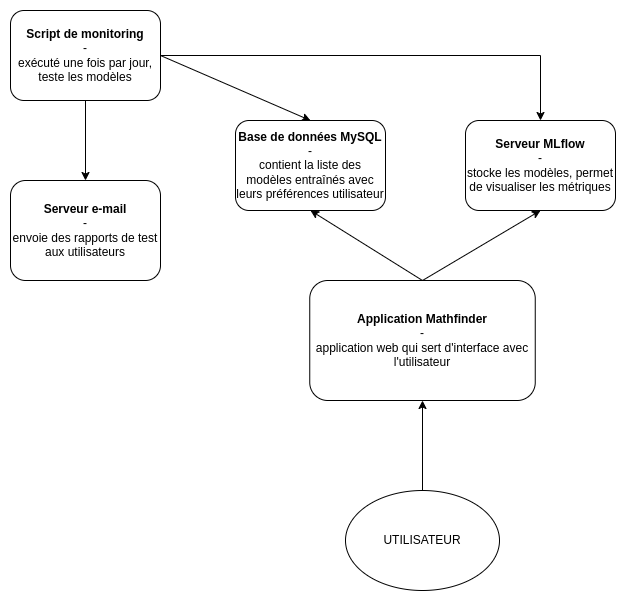
\includegraphics[width=10cm]{monitoring_E5}
        \centering
        \caption{Architecture de Mathfinder après avoir intégré un système de monitorage des modèles. Les flèches indiquent une relation d'usage (l'entité à l'origine de la flèche "utilise" celle vers laquelle la flèche se dirige)}
        \centering
        \label{fig:architecture}
    \end{figure}
    \begin{figure}[h!]
        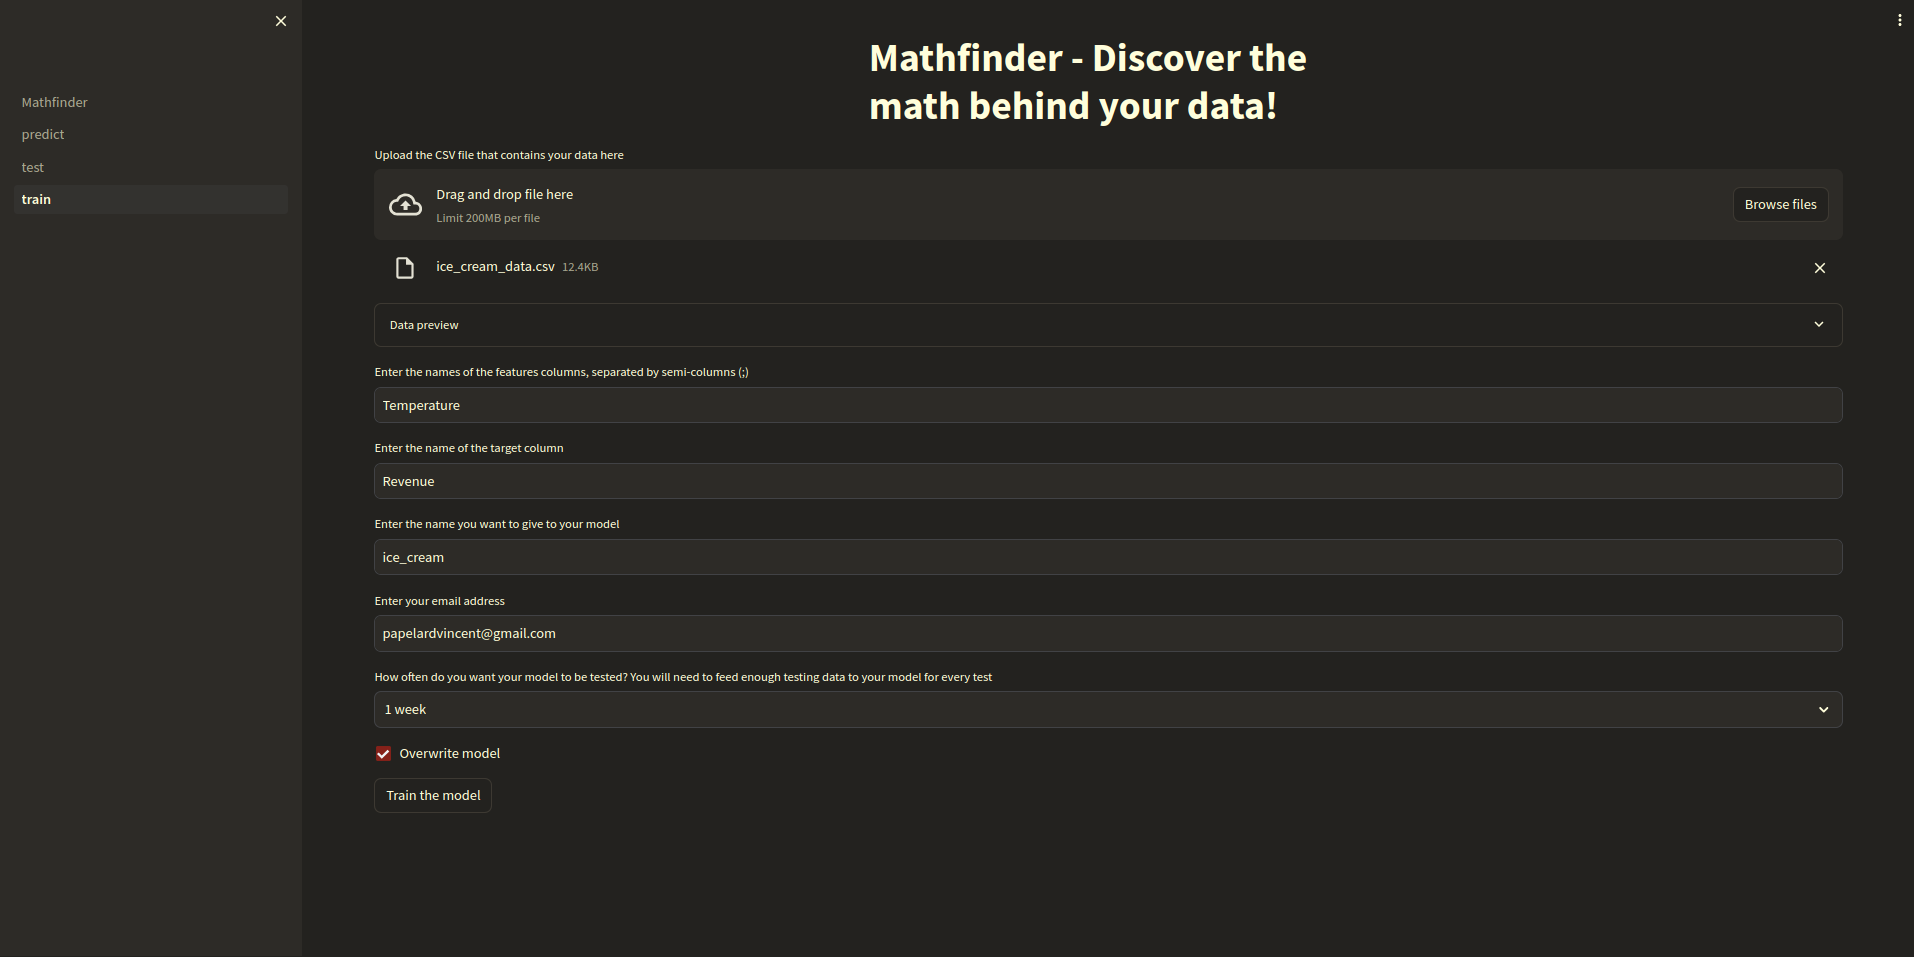
\includegraphics[width=10cm]{appli_2}
        \centering
        \caption{Page d'entraînement du modèle après avoir mis en place les mécanismes de suivi présentés dans ce dossier. On remarquera l'ajout de champs pour permettre à l'utilisateur de nommer son modèle, donner son adresse e-mail, spécifier une fréquence de test et décider d'écraser ou non les modèles déjà enregistrés qui ont le même nom}
        \centering
    \end{figure}
    \begin{figure}[h!]
        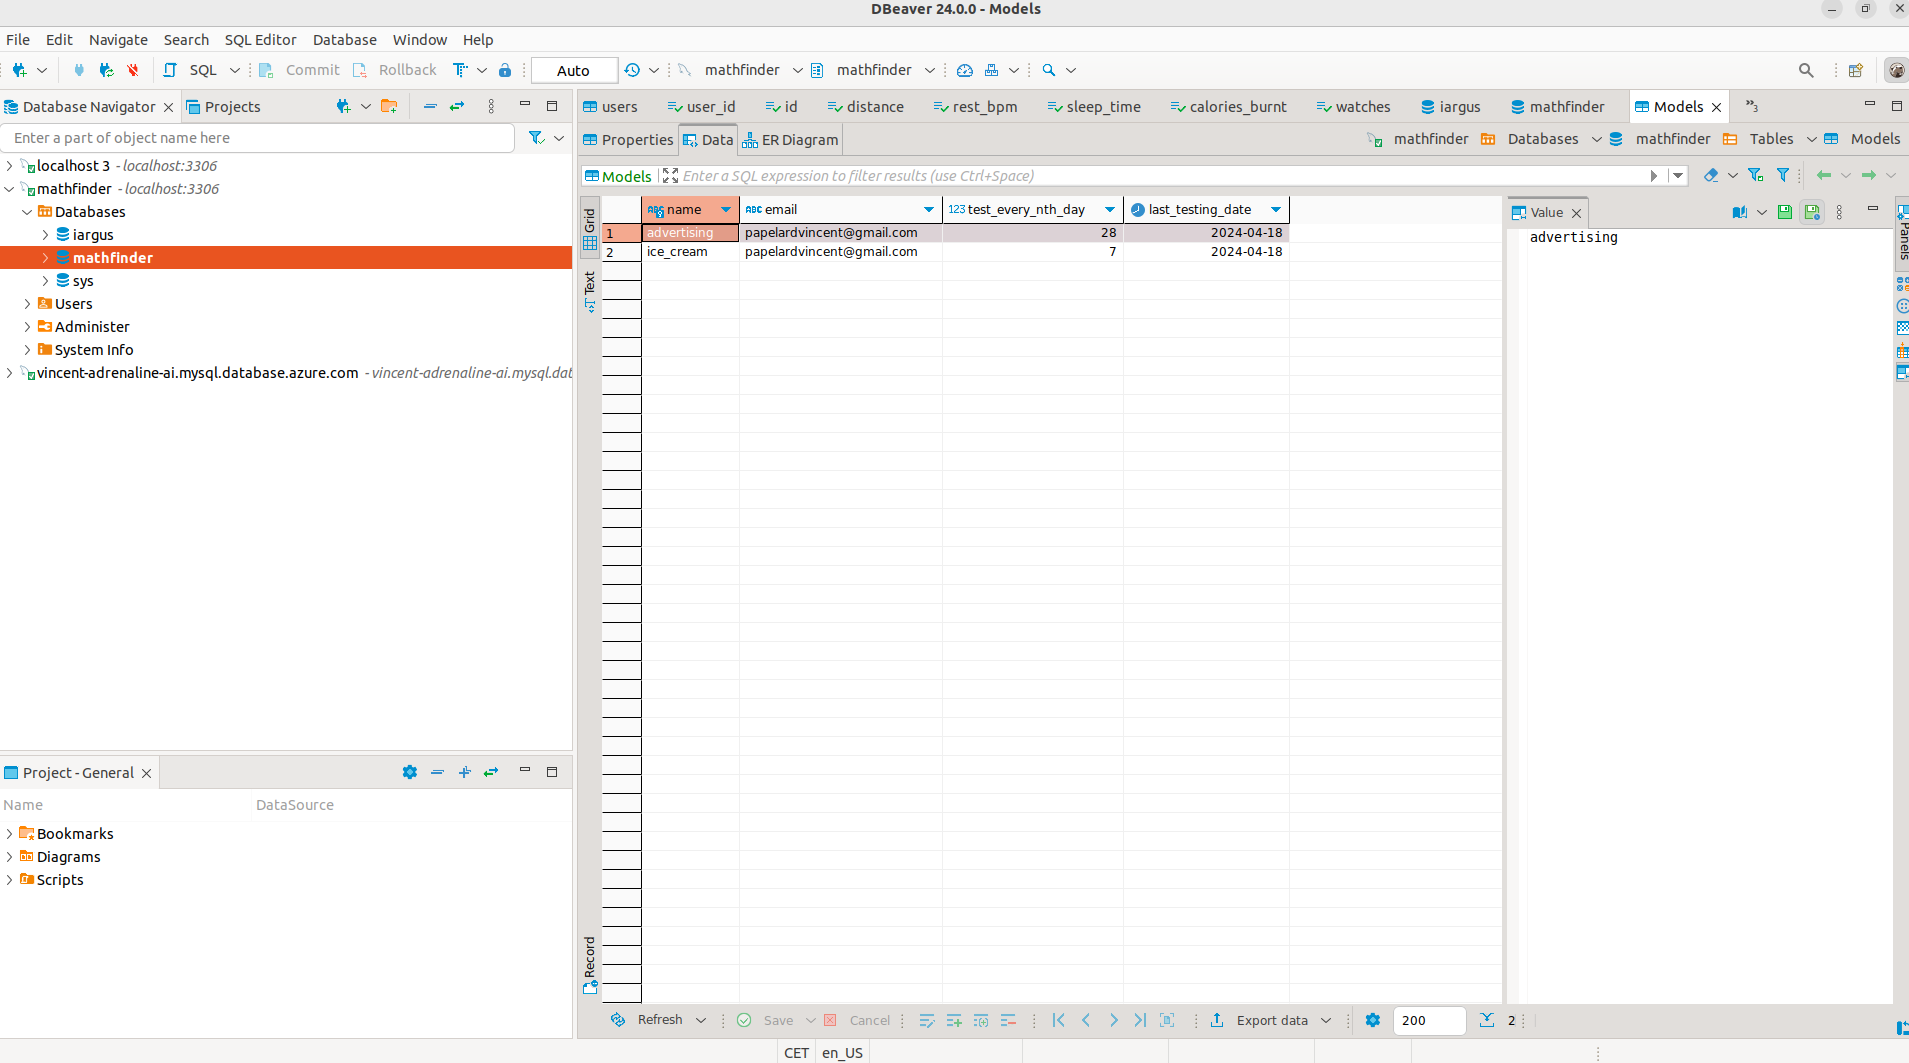
\includegraphics[width=10cm]{db}
        \centering
        \caption{Vue de la table "Models" de notre base de données sur DBeaver. Cette table stocke pour chaque modèle sa fréquence de test (choisie par l'utilisateur au moment de la création du modèle sur l'application), l'adresse e-mail à laquelle envoyer les rapports de test, ainsi que la date du dernier test réalisé}
        \centering
    \end{figure}
    \begin{figure}[h!]
        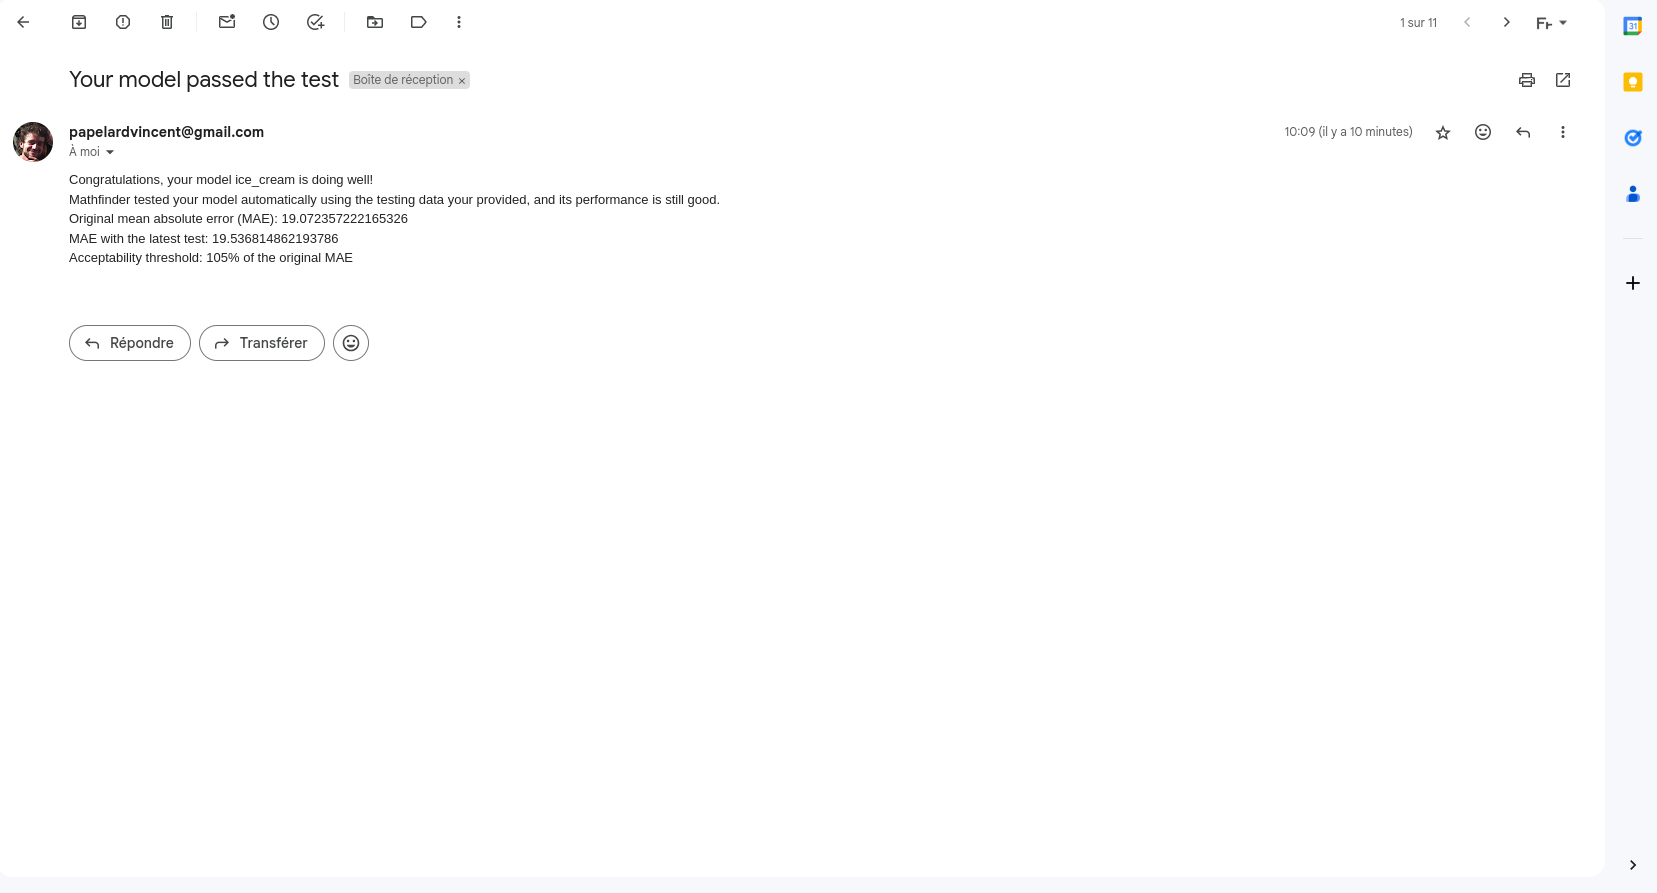
\includegraphics[width=10cm]{email_2}
        \centering
        \caption{Un rapport de test automatiquement envoyé par e-mail. Ici, le rapport de test nous indique que l'erreur absolue moyenne calculée pendant le test respecte la limite de 105 \% définie lors du premier entraînement du modèle. Remarque : l'adresse e-mail de l'expéditeur dépend du serveur SMTP utilisé pour envoyer l'e-mail. Le serveur de GMail ayant été utilisé ici, l'adresse de l'expéditeur est donc papelardvincent@gmail.com.}
        \centering
        \label{fig:email}
    \end{figure}
    \begin{figure}[h!]
        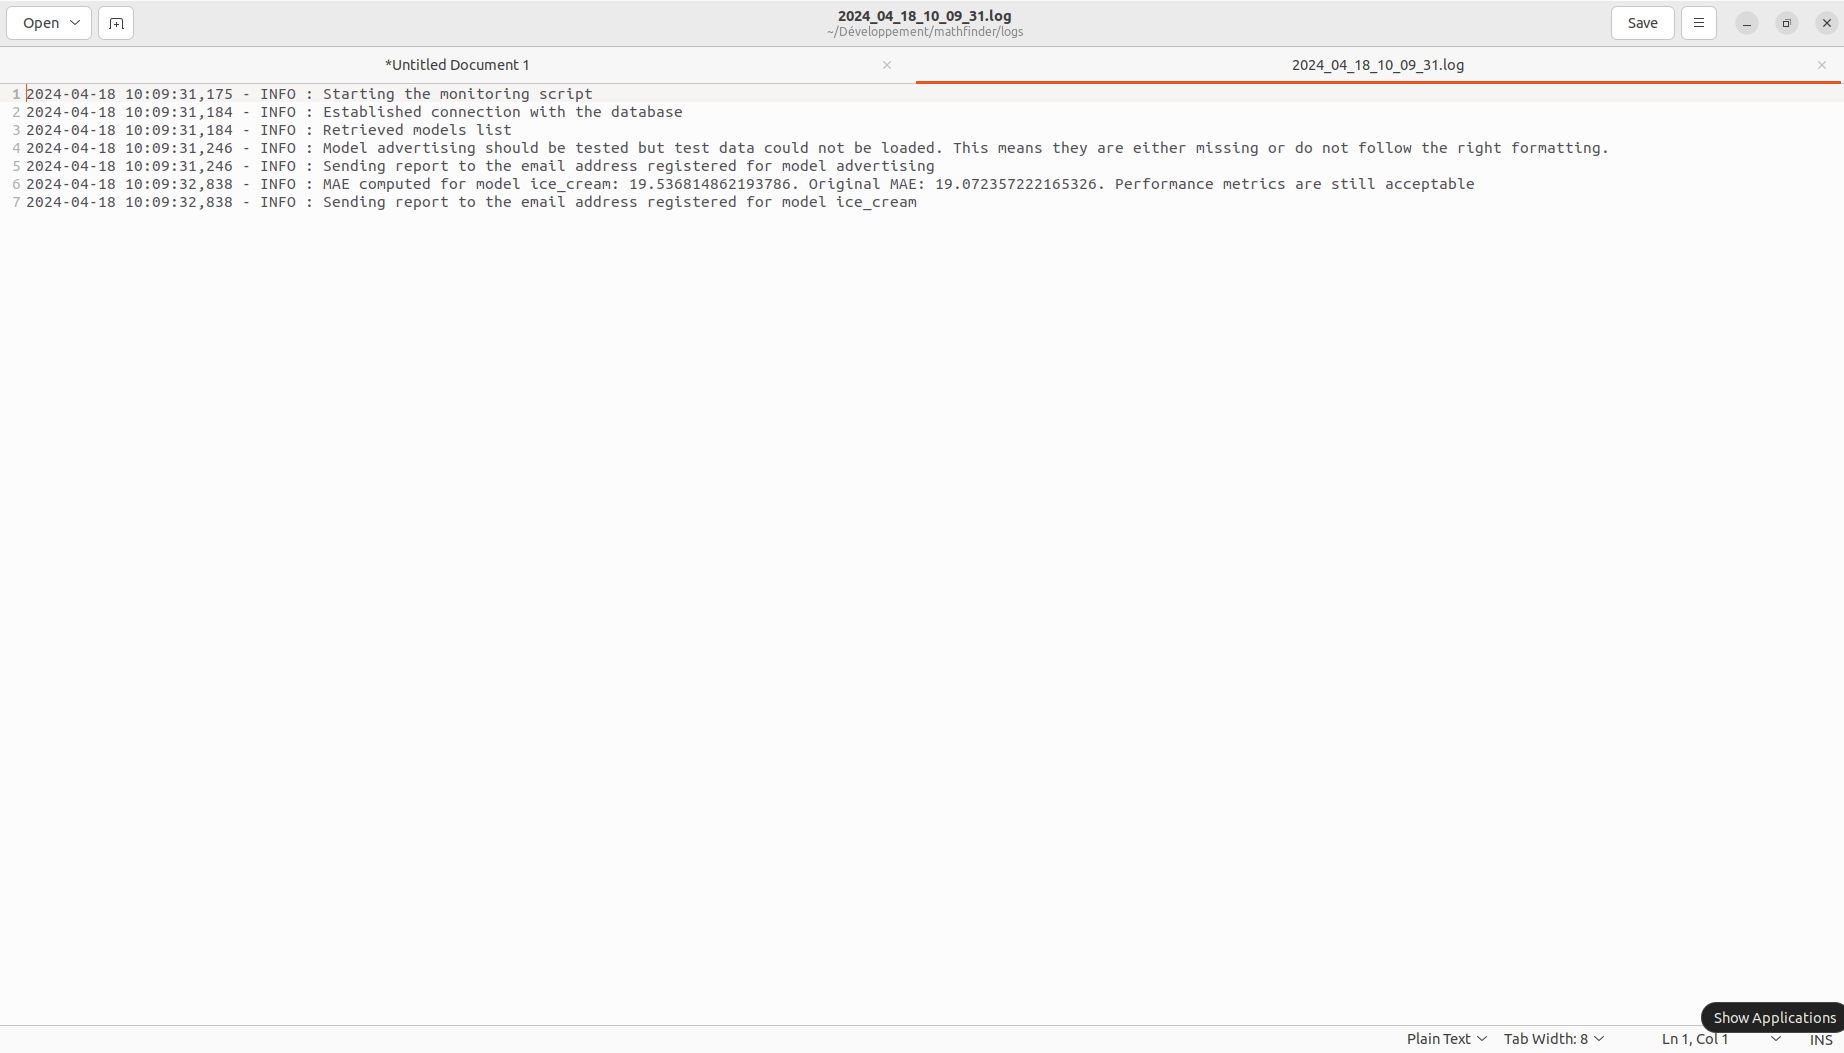
\includegraphics[width=10cm]{log}
        \centering
        \caption{Un exemple de fichier de journalisation généré par le script de monitorage de Mathfinder. Chaque message est accompagné de la date et l'heure correspondante afin de faciliter au maximum la lexture du fichier par les administrateurs.}
        \centering
    \end{figure}
    \begin{figure}[h!]
        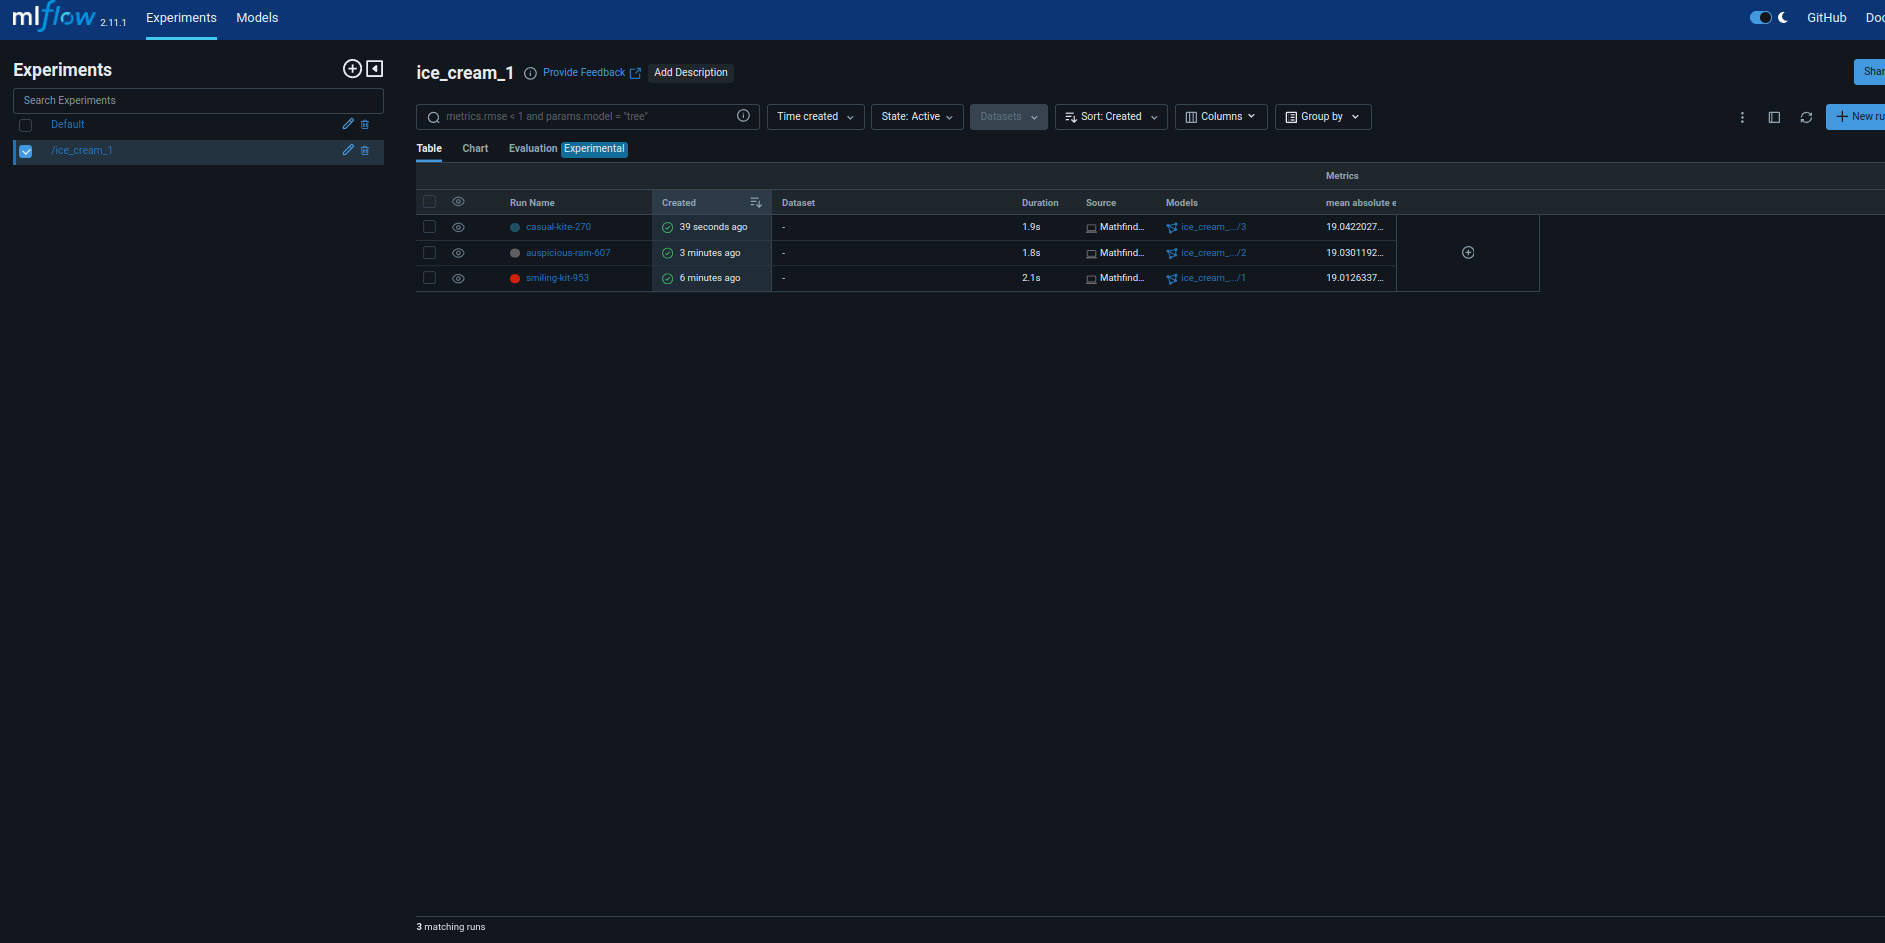
\includegraphics[width=10cm]{ml_flow_home}
        \centering
        \caption{Page d'accueil du tableau de bord MLflow. Le panneau de gauche liste les différents modèles suivis par MLflow (un seul dans ce cas) et le panneau de droite liste les différents entraînements et tests réalisés avec les métriques obtenues}
        \centering
    \end{figure}
    \begin{figure}[h!]
        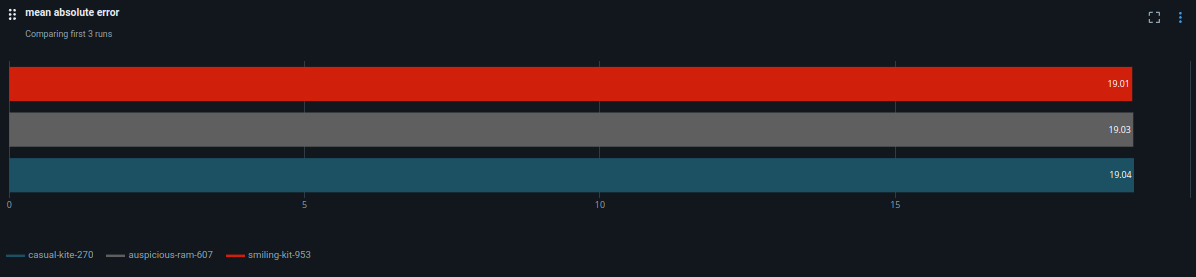
\includegraphics[width=10cm]{ml_flow_metrics}
        \centering
        \caption{Graphique généré par MLflow qui présente l'erreur absolue moyenne obtenue par un modèle lors de trois entraînements différents}
        \centering
        \label{fig:mlflow}
    \end{figure}
    \begin{figure}[h!]
        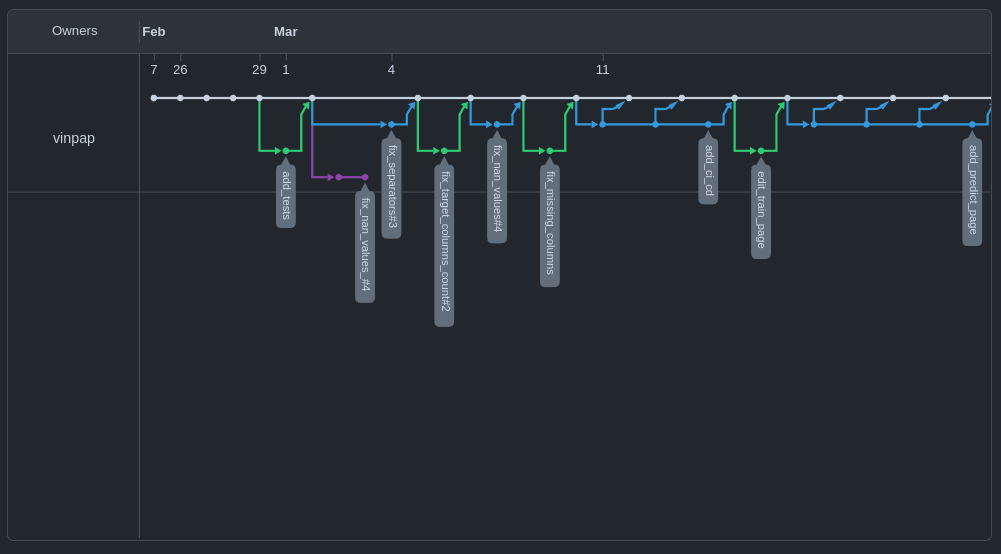
\includegraphics[width=10cm]{gh_graph}
        \centering
        \caption{Graphique généré par GitHub qui représente les branches du dépôt. De nouvelles branches sont créées pour traiter les problèmes techniques signalés via les tickets GitHub, ou pour ajouter des fonctionnalités nécessaires au monitorage du modèle. Les différentes branches sont intégrées à la branche principale du projet en utilisant des pull requests (demandes de fusion de branche)}
        \centering
    \end{figure}
    \begin{figure}[h!]
        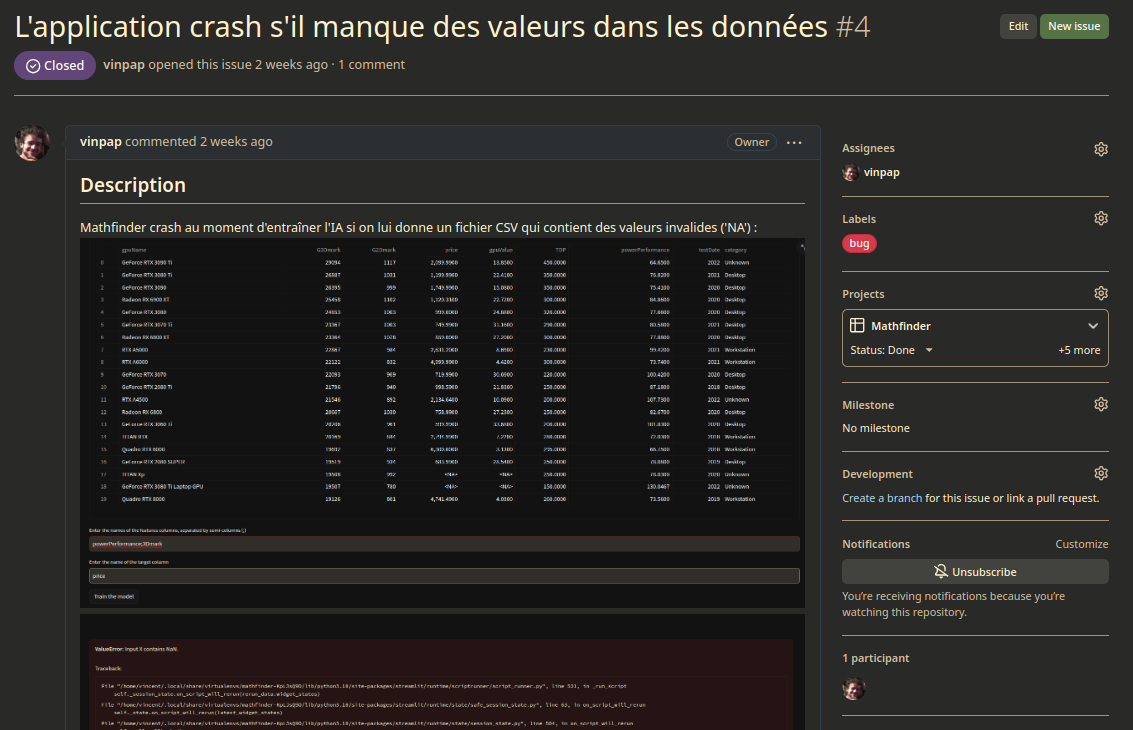
\includegraphics[width=10cm]{gh_issue}
        \centering
        \caption{Un exemple de ticket utilisé pour signaler un problème technique. Chaque ticket est accompagné d'une description du problème, des actions à réaliser pour le reproduire et de captures d'écran pour illustrer le problème}
        \centering
    \end{figure}
    \begin{figure}[h!]
        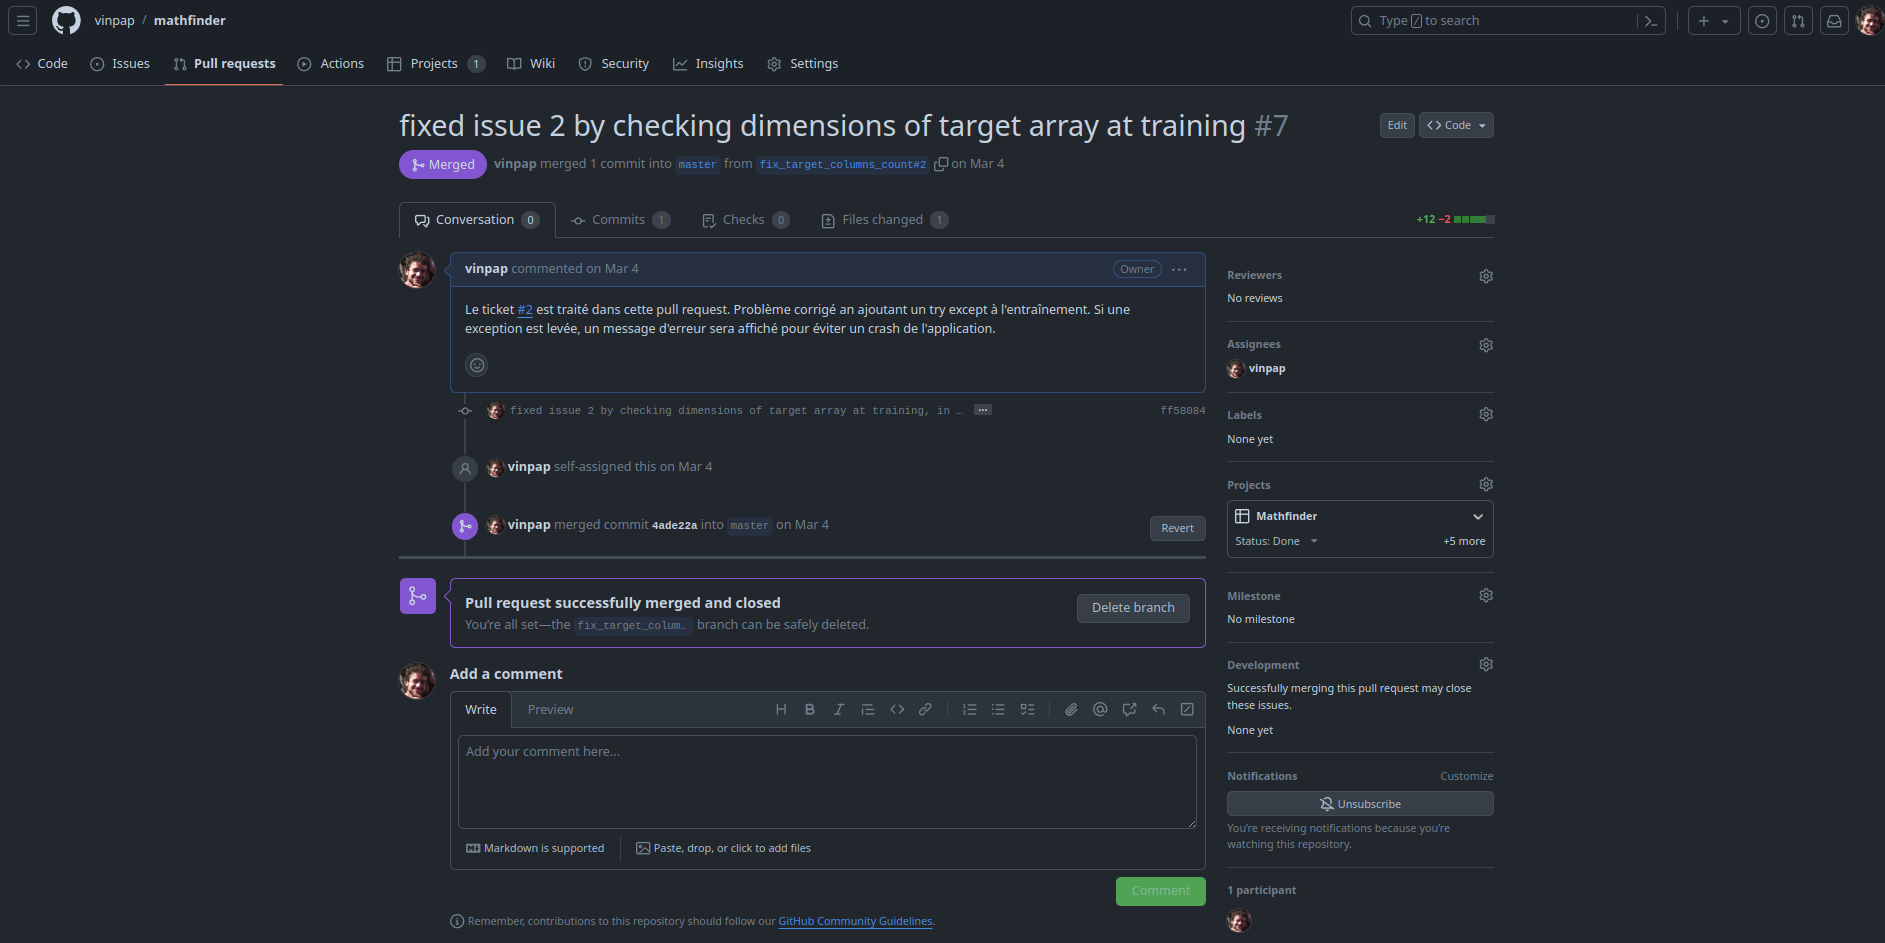
\includegraphics[width=10cm]{gh_pull_request}
        \centering
        \caption{Une pull request (demande de fusion de branche). Ici, la pull request explique quel problème technique a été réglé et explique comment. Une fois que la pull request est acceptée, le code de la branche d'origine est fusionné avec celui de la branche cible (ici la branche "master")}
        \centering
    \end{figure}
\end{document}